\documentclass{article}
\usepackage[utf8]{vietnam}
\usepackage[legalpaper, margin = 0.5in]{geometry}
\usepackage{multirow}
\usepackage{float}
\usepackage{graphicx}
\usepackage{caption}
\captionsetup{belowskip = 12pt, aboveskip = 12pt}
\graphicspath{{images/}}
\begin{document}
\begin{titlepage}
	\begin{center}
		%	\begin{tabular}{l}
		\large{\textbf{ĐẠI HỌC QUỐC GIA THÀNH PHỐ HỒ CHÍ MINH}}\\
		\large{\textbf{TRƯỜNG ĐẠI HỌC KHOA HỌC TỰ NHIÊN}}\\
		\large{\textbf{KHOA CÔNG NGHỆ THÔNG TIN}}\\
		%	\end{tabular}
		
		\begin{figure}[H]
			\centerline{
\includegraphics[scale = 0.5]{logo}}
		\end{figure}
		\vfill
		
		\large{\textbf{MÔN: XỬ LÝ ẢNH SỐ }}\\
		\large{\textbf{LỚP: CỬ NHÂN TÀI NĂNG 2013}}\\
	\end{center}
	\vfill
	\center{\Huge{\textbf{BÁO CÁO THỰC HÀNH - ĐỢT 2}}}
	
	\vfill
	
	\begin{flushright}
		\begin{tabular}{l l l}
			\textbf{GVLT}: & Thầy Lý Quốc Ngọc\\
			\textbf{GVTH}: & Thầy Võ Hoài Việt\\
			\textbf{Nhóm:} & Pixel\\
			\textbf{Thành viên}: & La Ngọc Thùy An & 1312716\\
			& Bùi Ngọc Bảo Ân & 1312020\\
			& Nguyễn Phan Mạnh Hùng & 1312727\\
		\end{tabular}
	\end{flushright}
\end{titlepage}
\pagebreak
\section{Tự cài đặt}
\begin{table}[H]
\begin{tabular}{l | l | l| p{3cm} }
	\hline
	\textbf{STT} & \textbf{Tên tác vụ} & \textbf{cài đặt? (Y/N)} & \textbf{File cài đặt} \\
	\hline
	\textbf{1} & \textbf{Nhóm tác vụ 01 - Hiển thị ảnh-video} & \\  \hline 
	1.1 & Đọc và hiển thị ảnh màu. &  Y & main.cpp \\ \hline 
	1.2 & Đọc và hiển thị ảnh độ sâu. & Y & depthimage\\ \hline 
	1.3 & Đọc và hiển thị video. & Y & video\\ \hline 
	1.4 & Chuyển đổi mô hình màu RGB $\to$ HSV và ngược lại. & Y & convert Color Model \\  \hline
	1.5 & Chuyển đổi mô hình màu RGB $\to$ LUV, Lab, YCbCr và ngược lại. & Y \\ \hline 
	\textbf{2} & \textbf{Nhóm tác vụ 02 - Hiệu chỉnh màu sắc} &\\ \hline 
	2.1 & Hiệu chỉnh màu sắc ảnh theo mô hình tuyến tính. & Y &  changecolor \\ \hline 
	2.2 & Hiệu chỉnh màu sắc ảnh theo mô hình phi tuyến. & Y & changecolor\\ \hline 
	2.3 & Hiệu chỉnh màu sắc ảnh theo mô hình thống kê. & Y & Histogram\\ \hline
	\textbf{3} & \textbf{Nhóm tác vụ 03 - Biến đổi hình học} & & \\ \hline 
	3.1 & Phép co giãn. & Y & Transform\\ \hline 
	3.2 & Phép xoay. & Y & Transform\\ \hline 
	\textbf{4} & \textbf{Nhóm tác vụ 04 - Tiền xử lý cục bộ} &\\ \hline 
	4.1 & Các toán tử làm trơn ảnh. &  Y & operator.h (median), kernel.h (gauss)  \\ \hline

	4.2 & Các toán tử phát hiện biên cảnh. & Y & EdgeDectector (canny), gradient (sobel, prewitt, freichen)\\ \hline
\end{tabular}
\end{table}

\section{Sử dụng thư viện}
	Hoàn tất
\section{Hình ảnh minh họa}

	\subsection{Nhóm tác vụ 01}
		\begin{figure}[H]
			\centering
			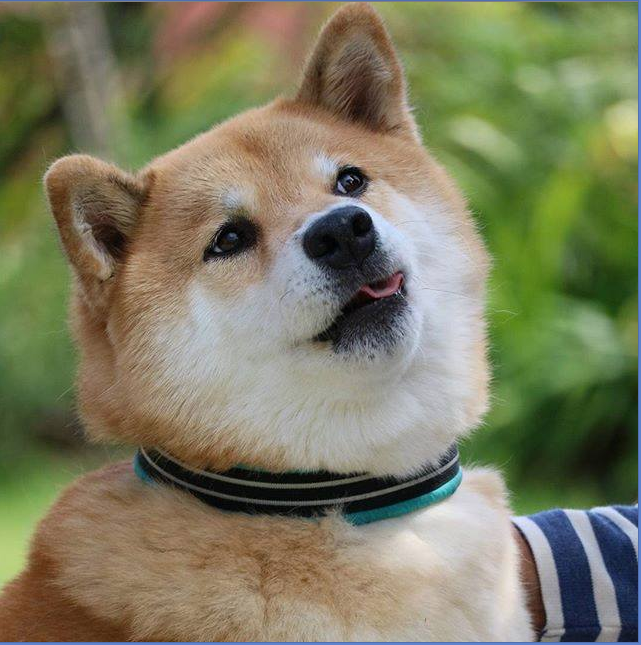
\includegraphics[scale = 0.4]{11show}
			\caption{Tác vụ 1.1: Hiển thị ảnh màu}
		\end{figure}
		\begin{figure}[H]
			\centering
			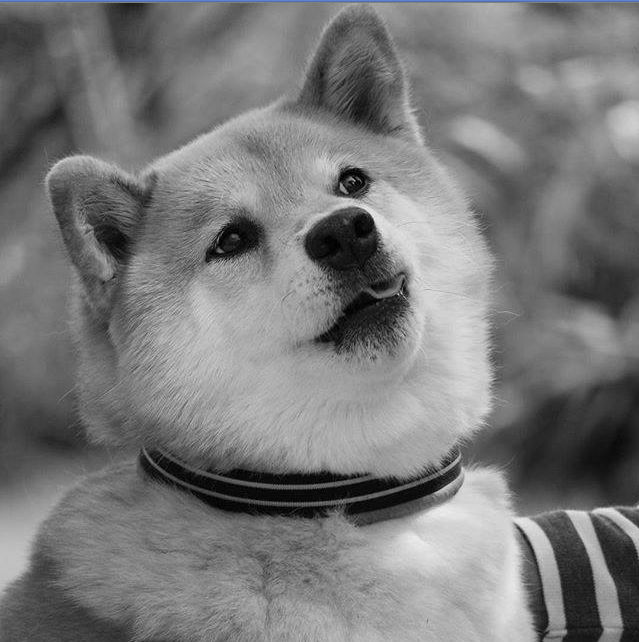
\includegraphics[scale = 0.4]{12depth}
			\caption{Tác vụ 1.2: Hiển thị ảnh độ sâu}
		\end{figure}
		\begin{figure}[H]
			\centering
		%	\includegraphics[scale = 0.4]{13}
		%	\caption{Tác vụ 1.3}
		\end{figure}
		\begin{figure}[H]
			\centering
			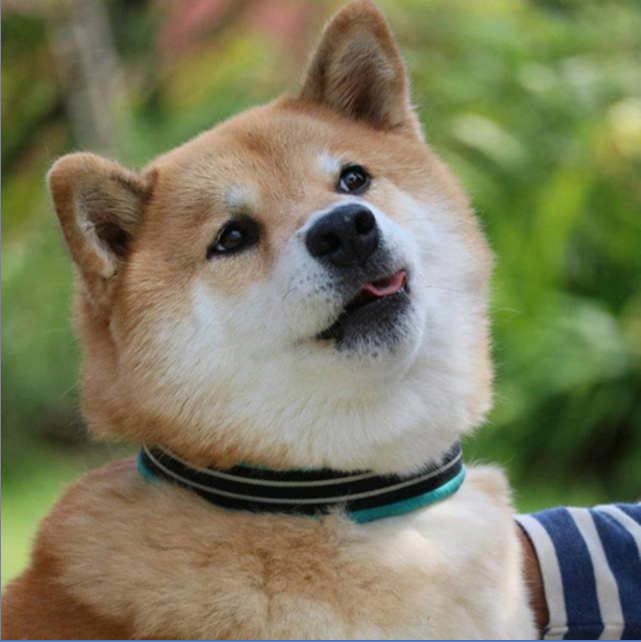
\includegraphics[scale = 0.4]{14}
			\caption{Tác vụ 1.4: RGB - HSV}
		\end{figure}
		\begin{figure}[H]
			\centering
			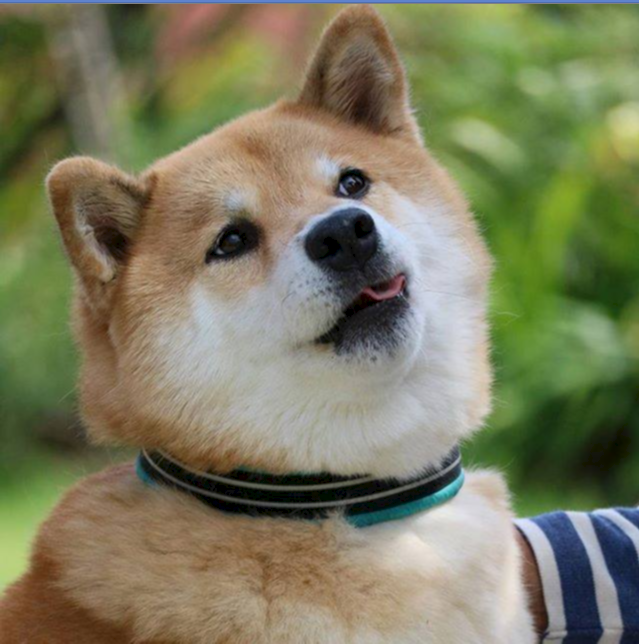
\includegraphics[scale = 0.4]{15luv}
			\caption{Tác vụ 1.5: RGB - LUV}
		\end{figure}
		\begin{figure}[H]
			\centering
			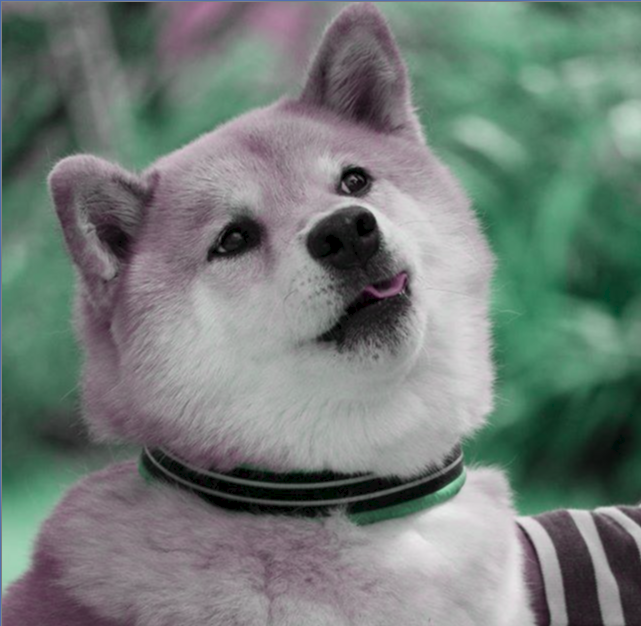
\includegraphics[scale = 0.4]{15lab}
			\caption{Tác vụ 1.5: RGB - LAB}
		\end{figure}
		\begin{figure}[H]
			\centering
			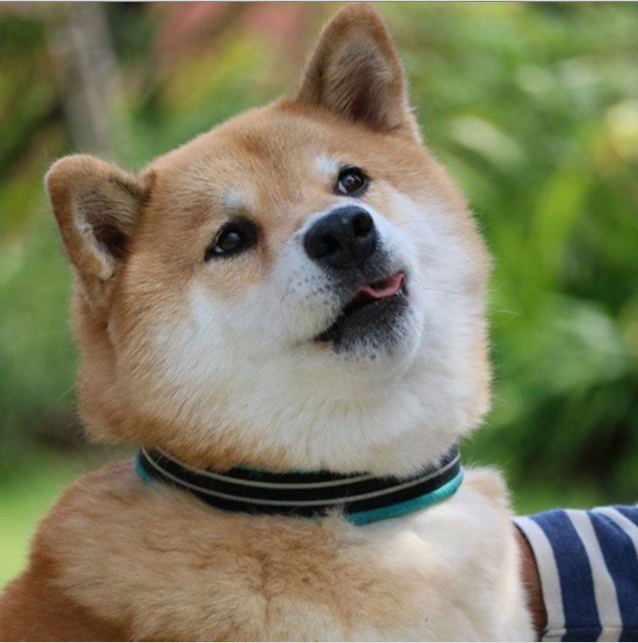
\includegraphics[scale = 0.4]{15ycbcr}
			\caption{Tác vụ 1.5: RGB - YCBCR}
		\end{figure}
	\subsection{Nhóm tác vụ 02}
	\begin{figure}[H]
		\centering
		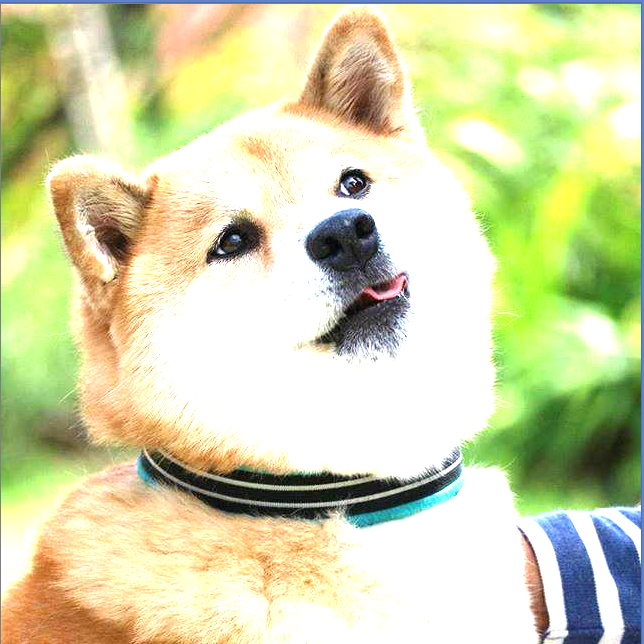
\includegraphics[scale = 0.4]{21linear}
		\caption{Tác vụ 2.1: Hiệu chỉnh màu mô hình tuyến tính}
	\end{figure}
	\begin{figure}[H]
		\centering
		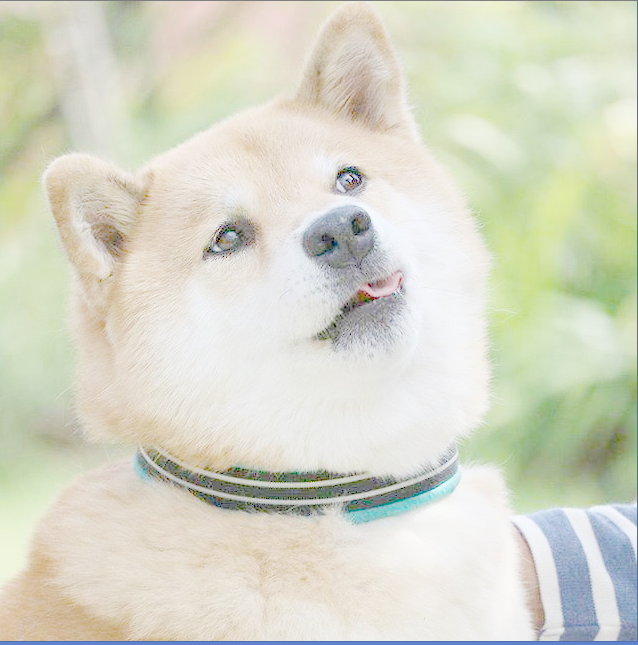
\includegraphics[scale = 0.4]{22log}
		\caption{Tác vụ 2.2: Non-linear transformation (log)}
	\end{figure}
		\begin{figure}[H]
			\centering
			
\includegraphics[scale = 0.4]{22e}
			\caption{Tác vụ 2.2: Non-linear transformation (exponential)}
		\end{figure}
	\begin{figure}[H]
		\centering
		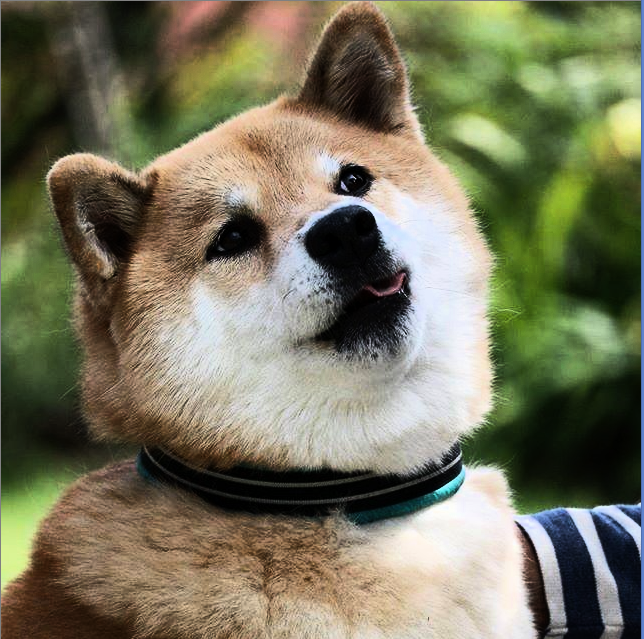
\includegraphics[scale = 0.4]{23histogram}
		\caption{Tác vụ 2.3: Hiệu chỉnh màu mô hình thống kê}
	\end{figure}
	
	\subsection{Nhóm tác vụ 03}
	\begin{figure}[H]
		\centering
		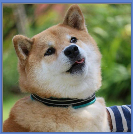
\includegraphics[scale = 0.4]{31zoom}
		\caption{Tác vụ 3.1: Co giãn}
	\end{figure}
	\begin{figure}[H]
		\centering
		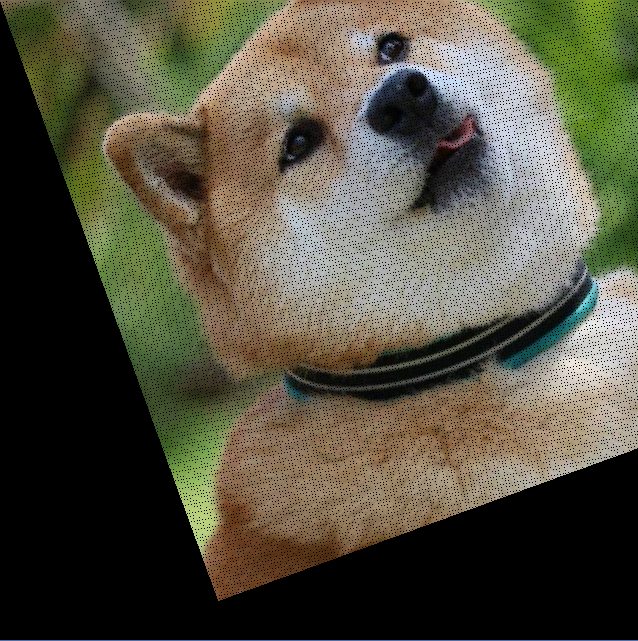
\includegraphics[scale = 0.4]{32rotation}
		\caption{Tác vụ 3.2: Rotate}
	\end{figure}

	\subsection{Nhóm tác vụ 04}
	\begin{figure}[H]
		\centering
		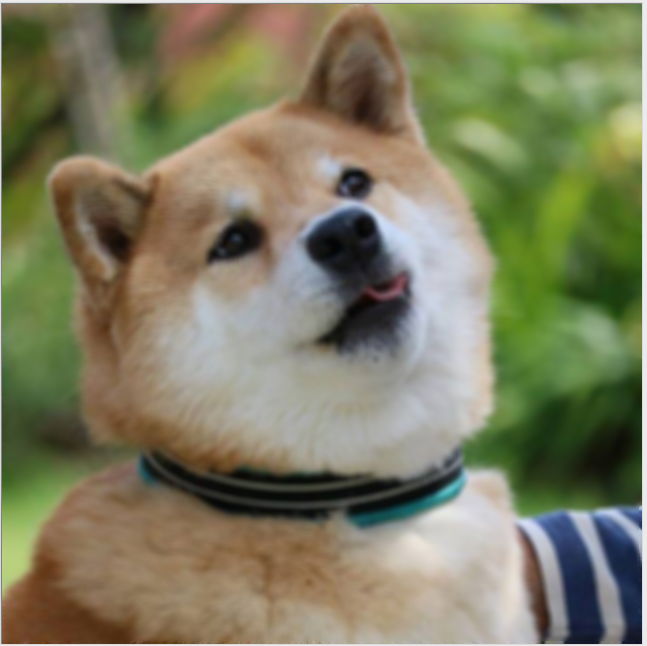
\includegraphics[scale = 0.4]{41mean}
		\caption{Tác vụ 4.1: Toán tử trung bình}
	\end{figure}
	\begin{figure}[H]
		\centering
		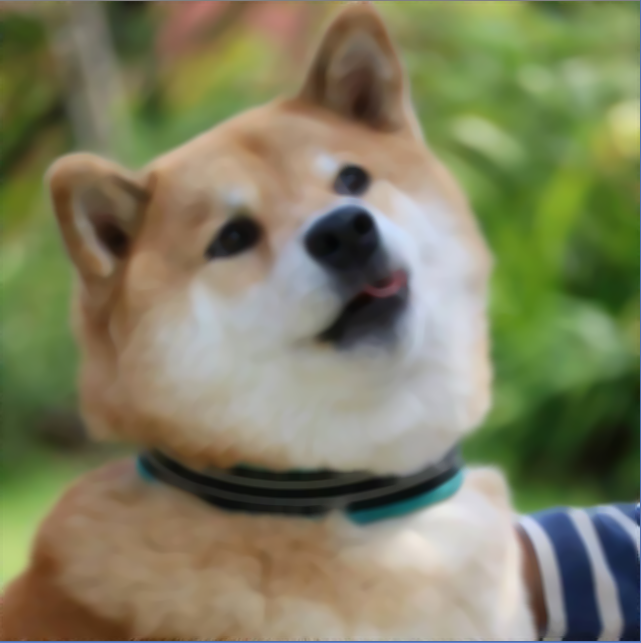
\includegraphics[scale = 0.4]{41median}
		\caption{Tác vụ 4.1: Toán tử trung vị}
	\end{figure}
	\begin{figure}[H]
		\centering
		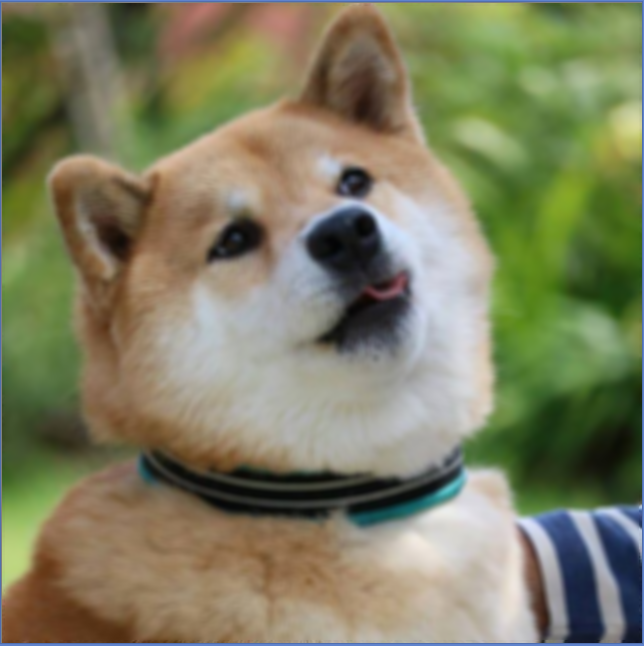
\includegraphics[scale = 0.4]{41gauss}
		\caption{Tác vụ 4.1: Toán tử Gauss}
	\end{figure}
	\begin{figure}[H]
		\centering
		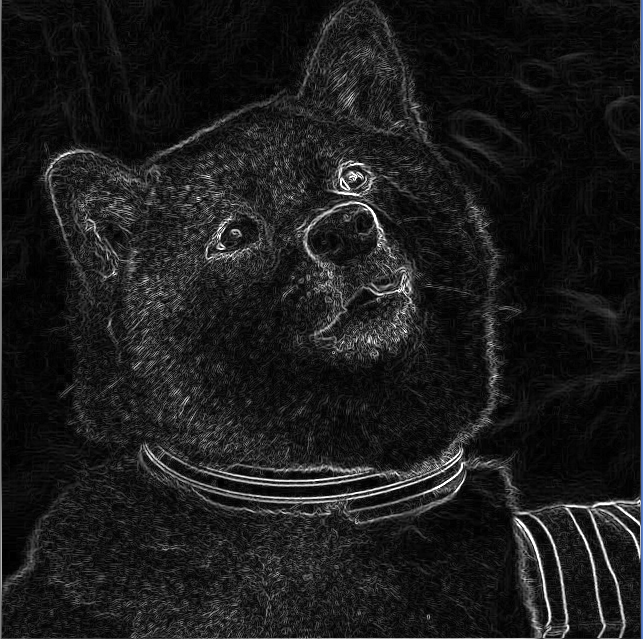
\includegraphics[scale = 0.4]{42sobel}
		\caption{Tác vụ 4.2: Sobel}
	\end{figure}
		\begin{figure}[H]
			\centering
			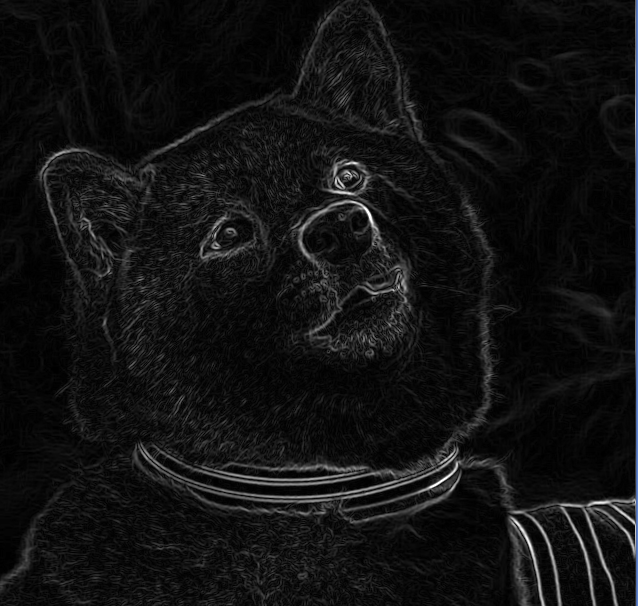
\includegraphics[scale = 0.4]{42freichen}
			\caption{Tác vụ 4.2: Freichen}
		\end{figure}
		\begin{figure}[H]
			\centering
			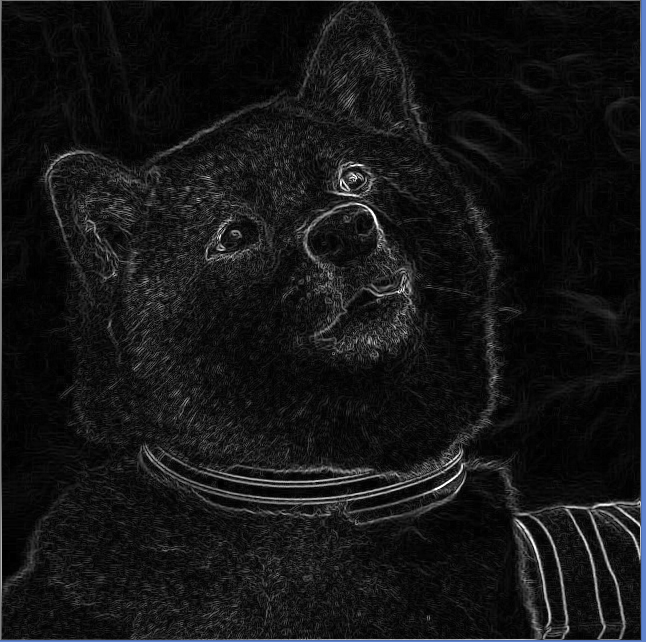
\includegraphics[scale = 0.4]{42prewitt}
			\caption{Tác vụ 4.2: Prewitt}
		\end{figure}
	\begin{figure}[H]
		\centering
		\includegraphics[scale = 0.4]{42canny}
		\caption{Tác vụ 4.2: Canny}
	\end{figure}
%\section{Đánh giá}
%	Tốc độ xử lý của hàm convolution chưa đạt yêu cầu (khá chậm với ảnh có độ phân giải cao).\\
%	Bên cạnh đó, mô hình canny (tự cài đặt) dù phát hiện ra được các biên cạnh chính, nhưng đối với các chi tiết nhỏ và có biên không rõ thì thuật toán cho ra các đường đứt nét.
\end{document}